\appendix
\let\stdsection\section
\renewcommand\section{\newpage\stdsection}
\renewcommand{\thesection}{\Alph{section}}
\renewcommand*{\sectionmark}[1]{\markright{\MakeMarkcase{Anhang \thesection: #1}}}
\addcontentsline{toc}{chapter}{Anhang}

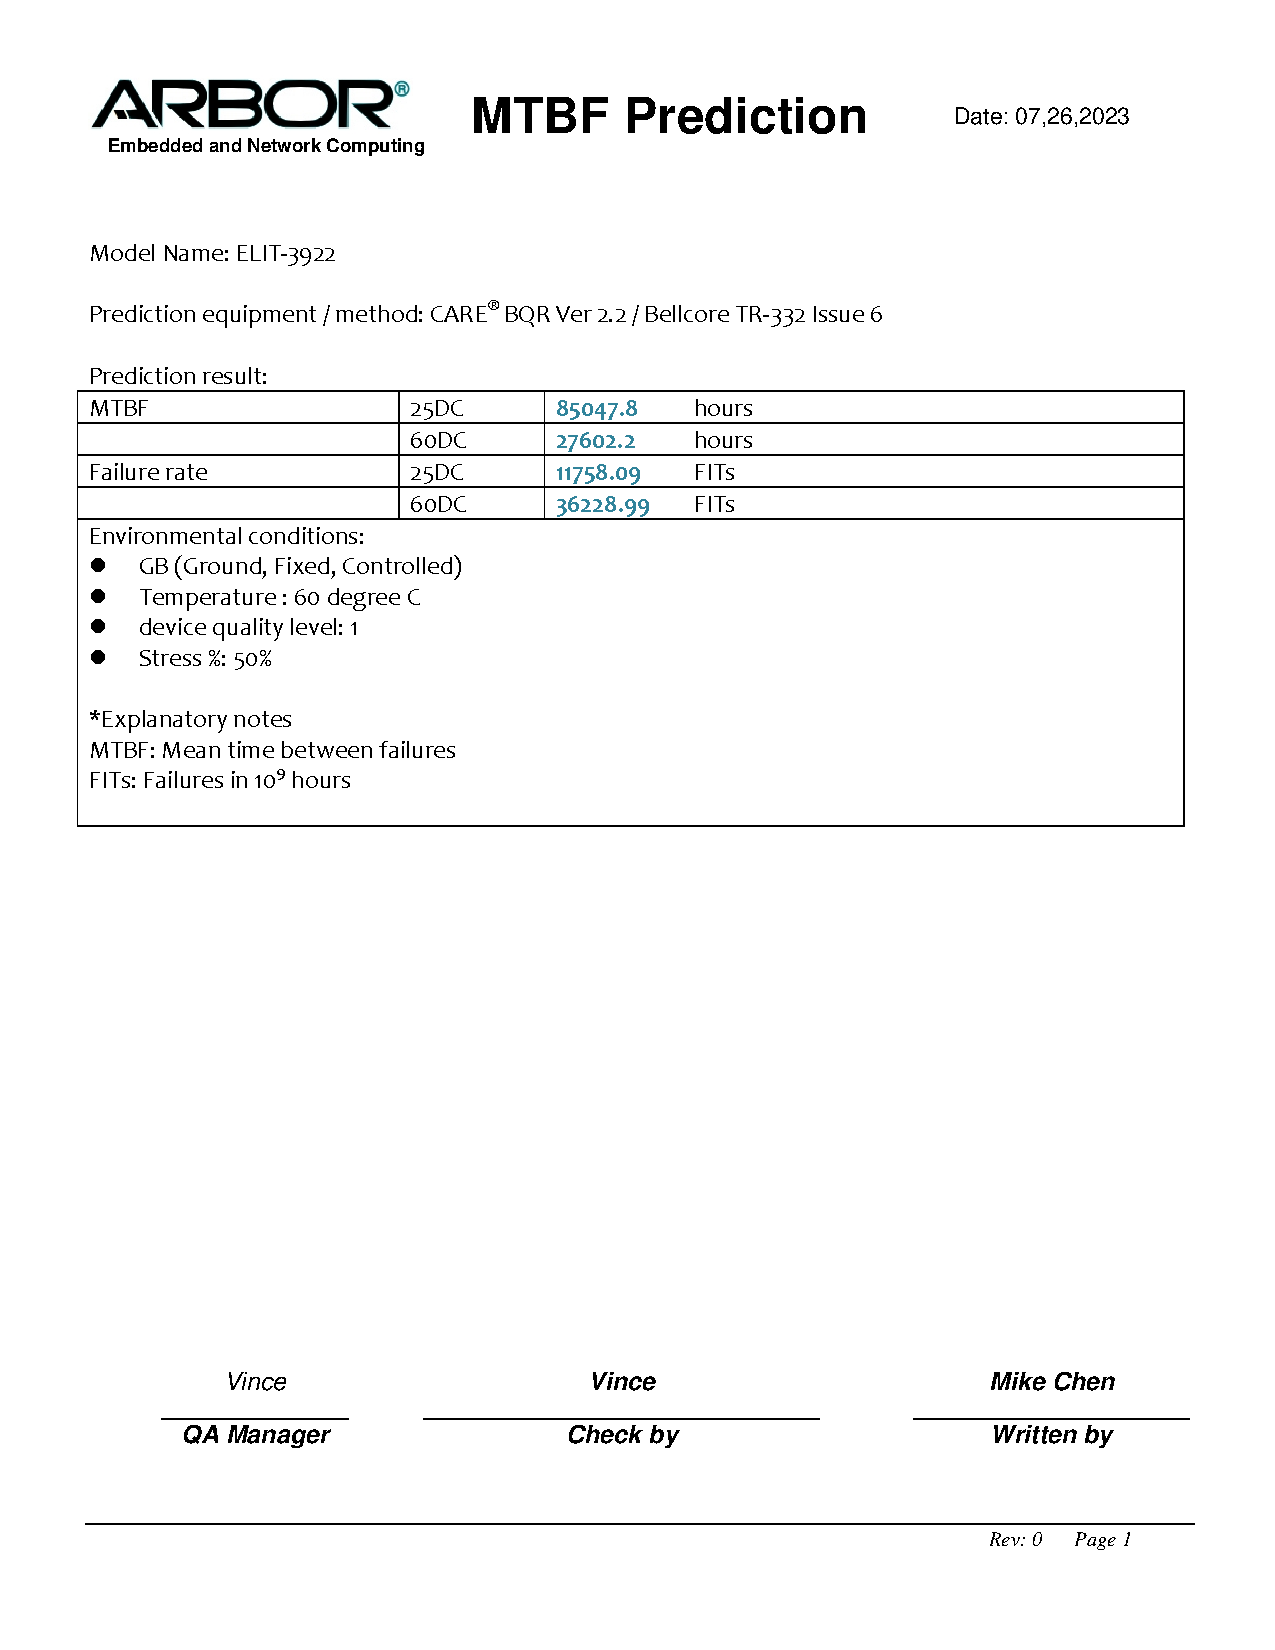
\includepdf[pages=-,scale = 0.8,
  pagecommand={},
  addtotoc={1,section,1,{MTBF Prediction VisuNet FLX},{app:mtbfprediction}}
]{sections/appendix/ELIT-3922-3965U_MTBF.PDF}




%\lstset{
%    captionpos=top,
%    language=C++,
%    backgroundcolor=\color{white}
%}

%Verbindung
%\section{Quellcode MQTT und WiFi Verbindung}\label{sec:bib_mqtt_wlan}

\section{Datenbank Konfiguration}\label{app:dbKonfiguration}
\lstinputlisting[label={lst:dbConfig},caption = Datenbank Konfiguration]{sections/appendix/HealthMonitoringDataBase.sql}

